% Project proposal: comparing LLMs on patient portal messages.
% Build: latexmk -pdf main.tex   (or: pdflatex main && pdflatex main)

\documentclass[11pt]{article}
\usepackage[preprint]{acl}

\usepackage{times}
\usepackage{latexsym}
\usepackage[T1]{fontenc}
\usepackage[utf8]{inputenc}
\usepackage{microtype}
\usepackage{inconsolata}
\usepackage{graphicx}
\usepackage{booktabs}
\usepackage{tabularx}
\usepackage{array}
\usepackage{enumitem}
\usepackage{xcolor}
\usepackage{tikz}
\usepackage{pgfplots}
\pgfplotsset{compat=1.17}
\usetikzlibrary{positioning,arrows.meta,shapes.geometric}

\definecolor{accent}{HTML}{2B6CD4}
\definecolor{muted}{HTML}{BDBDB3}
\definecolor{edge}{HTML}{8A8A80}
\definecolor{quiet}{HTML}{5F5F5F}

\setlist{nosep,leftmargin=*}
\newcolumntype{L}[1]{>{\raggedright\arraybackslash}p{#1}}
\newcolumntype{Y}{>{\raggedright\arraybackslash}X}

\title{Comparing Large Language Models on Patient Portal Messages:\\
Baselines, Chart Grounding, and Multi-Turn Evaluation}

\author{Lubna Zaman Lamia \\ Dartmouth College \And
  Jialin Yang \\ Dartmouth College \And
  Sudarshan Regmi \\ Dartmouth College}

\begin{document}
\maketitle


% ---------------------------------------------------------------------------
\section{Problem, Motivation, and Social Impact}

Patients send many messages to their care team through online portals.
Clinicians must read each message and reply.
This work takes time and adds to clinician burnout.

Many patient messages do not have enough detail.
For example, a patient writes ``I have a runny nose. What should I do?''
Before the clinician can help, the clinician must ask more questions.
Each round of questions adds delay for the patient.

LLMs can draft follow-up questions and replies, and health systems already test this.
But an LLM can make serious mistakes.
It can miss a warning sign, invent a fact, or give advice that is not safe.
It can also write at a reading level that is too hard for the patient.

There are many LLMs, and new ones come out often.
A health team needs a clear way to compare them on its own messages.
This project gives that method and a tool to apply it.
The potential social impact is:
\begin{itemize}
  \item \textbf{Faster care.} Good follow-up questions can collect the needed facts in the first reply.
  \item \textbf{Less clinician workload.} A good draft can save time on routine messages.
  \item \textbf{Safer adoption.} A clear comparison shows where models fail before a team uses them with real patients.
  \item \textbf{Better access.} Plain-language replies help patients with lower health literacy.
\end{itemize}

% ---------------------------------------------------------------------------
\section{Users, Stakeholders, and Use Context}

The tool is for people who must decide if and how to use an LLM for patient messages.
It is not for patients to use directly.
Table~\ref{tab:users} lists the groups.

\begin{table}[t]
\centering\small
\begin{tabularx}{\columnwidth}{@{}L{2.3cm}Y@{}}
\toprule
\textbf{Group} & \textbf{Role and need} \\
\midrule
Clinical informatics teams & Primary users. Need a fair comparison of models on their own messages. \\
Clinicians & Raters, authors of the reference answers, and end readers. Need drafts that are safe, correct, and save time. \\
Researchers & Users. Need a repeatable method and exportable results. \\
Patients & Affected stakeholders. Need clear, safe, and timely replies. \\
Health system leaders & Decision makers. Need evidence about risk and benefit. \\
\bottomrule
\end{tabularx}
\caption{Users and stakeholders.}
\label{tab:users}
\end{table}

\paragraph{Use context.}
A user runs the app on a local computer.
The user picks a de-identified message, selects models and baselines, and reads the outputs side by side.
A clinician can score the outputs blind on a separate page.
The user can also hold a multi-turn chat, or run a simulated one.
No model output goes to a real patient.

% ---------------------------------------------------------------------------
\section{Research Questions and System Objective}

\paragraph{System objective.}
Build a web app that runs several LLMs and baselines on the same patient message, scores each output, and shows the results side by side.

\noindent We ask four research questions:
\begin{enumerate}
  \item \textbf{RQ1 -- Quality.} How well do current LLMs write clinician-like follow-up questions and replies? How do they compare to simple retrieval and checklist baselines?
  \item \textbf{RQ2 -- Chart context.} Does the chart summary (EHR) make the outputs better? Do the outputs stay true to the chart? We run each model with and without it.
  \item \textbf{RQ3 -- Evaluation.} Do the cheap automatic metrics and the LLM judge agree with each other, with the clinician reference answers, and with ratings from the app's blind rating page?
  \item \textbf{RQ4 -- Multi-turn.} In a conversation, how fast does a model collect the facts a clinician would ask for? Does it notice a warning sign that appears in a later turn?
\end{enumerate}

% ---------------------------------------------------------------------------
\section{Methods and Baselines}

\paragraph{Tasks.} The system supports three tasks:
\begin{itemize}
  \item \textbf{Follow-up questions.} Input: a patient message and a chart summary. Output: a numbered list of questions.
  \item \textbf{General reply.} Input: the same. Output: a short, plain-language reply.
  \item \textbf{Multi-turn conversation.} The model talks with a patient over several turns. It asks questions, gets answers, and then gives advice.
\end{itemize}

\paragraph{LLM method.}
We use zero-shot prompting.
Every model gets the same system prompt and the same input, so the comparison is fair.
The prompt tells the model not to diagnose, to give emergency advice when needed, and to use the chart summary.
We call all models through one API (OpenRouter).
We test the newest general model from five providers: OpenAI, Anthropic, Google, Meta, and Mistral.

\paragraph{Baselines.}
A strong LLM result means little without a simple point of comparison.
The baselines in Table~\ref{tab:baselines} run inside the app, next to the LLMs, and need no API call.
The retrieval baselines use leave-one-out: a message never retrieves its own answer.
So every message can serve as a test case, and no answer leaks into its own score.

\begin{table}[t]
\centering\small
\begin{tabularx}{\columnwidth}{@{}L{1.75cm}L{1.3cm}Y@{}}
\toprule
\textbf{Baseline} & \textbf{Type} & \textbf{How it works} \\
\midrule
Fixed checklist & Symbolic & Ask the same 8 general questions for every message (onset, severity, medications, \ldots). For replies, use one fixed template. \\
TF-IDF retrieval & Statistical & Find the most similar other message by TF-IDF cosine similarity. Return the clinician's questions or reply for it. \\
BM25 retrieval & Statistical & The same, with BM25 ranking instead of TF-IDF. \\
No chart summary & Ablation & Run each LLM with the message only. This isolates the effect of the EHR. \\
\bottomrule
\end{tabularx}
\caption{Baselines. None of them calls an LLM.}
\label{tab:baselines}
\end{table}

\paragraph{Multi-turn method.}
A second LLM plays the patient.
It sees one dataset message and its chart summary, and it answers only from them.
The assistant model then talks with this simulated patient for up to 6 turns.
In some runs, we add a warning sign (for example, chest pain) in a later patient turn.
This tests if the assistant notices it.

\paragraph{Planned extension.}
If time allows, we add few-shot prompting.
We put two or three clinician examples in the prompt and measure the change.

% ---------------------------------------------------------------------------
\section{Dataset and Data Sample}

We use two datasets of patient portal messages (Table~\ref{tab:data}).
Clinicians wrote the reference answers.
Each row also has a de-identified chart summary with age range, sex, problem list, diagnoses, and medications.
The two files share messages.
After we merge them, there are 227 unique messages.
All 227 have clinician questions, and 91 of them also have a clinician reply.

\begin{table}[t]
\centering\small
\begin{tabularx}{\columnwidth}{@{}lrY@{}}
\toprule
\textbf{File} & \textbf{Rows} & \textbf{Reference for} \\
\midrule
\texttt{questions.csv} & 250 & Follow-up questions \\
\texttt{responses.csv} & 100 & General reply \\
\bottomrule
\end{tabularx}
\caption{Datasets. Both include the message and the chart summary.}
\label{tab:data}
\end{table}

\paragraph{Representative sample} (chart summary shortened).
\begin{itemize}
  \item \textbf{Chart summary:} Age 40--45, female. Problems include migraine, dermatitis, and persistent depressive disorder.
  \item \textbf{Patient message:} ``I'm not feeling great today. I just started getting a really runny nose and I've been sneezing nonstop. I was wondering if I could get some advice on what to do.''
  \item \textbf{Clinician questions:} Do you have a fever? Have you been experiencing a headache? Do you have any cough? Have you tried any OTC medications? Have you been around anyone who has been sick with a viral illness?
  \item \textbf{Clinician reply:} ``I'm sorry you have been experiencing these troubling symptoms. Have you had any sick contacts recently? \ldots\ If your symptoms persist, or are getting worse, please call the office to schedule an appointment.''
\end{itemize}

% ---------------------------------------------------------------------------
\section{Initial Data Exploration}

We profiled both files (Table~\ref{tab:lengths}).
The main findings are below.

\begin{table}[t]
\centering\small
\begin{tabular}{@{}lrr@{}}
\toprule
\textbf{Text field} & \textbf{Median} & \textbf{Range} \\
\midrule
Chart summary & 180 & 37--303 \\
Patient message & 96 & 25--218 \\
Clinician questions & 63 & 15--227 \\
Clinician reply & 63 & 17--125 \\
\bottomrule
\end{tabular}
\caption{Length of each text field, in words.}
\label{tab:lengths}
\end{table}

\begin{itemize}
  \item \textbf{Clinicians ask about 9 questions per message.} The median is 9, and the range is 2 to 23. So a good model must ask several questions, but not too many.
  \item \textbf{The chart summary is longer than the message.} It is about twice as long, and most of it does not relate to the message. A model must find the few facts that matter.
  \item \textbf{Clinician replies are short and easy to read.} The median reading level is US grade 7.3 (Flesch-Kincaid). This gives us a target for LLM replies.
  \item \textbf{Clinician replies show empathy and safety.} 99 of 100 replies use empathetic words. 54 of 100 give emergency or urgent-care advice.
  \item \textbf{Some topics are common and some are rare.} We tagged the clinician questions with 8 clinical topics (Figure~\ref{fig:topics}). Clinicians screen for red flags in 57\% of messages. A model that skips this check fails a key safety step.
  \item \textbf{The patient group is not balanced.} 184 of 250 rows (74\%) are female. Ages range from 20 to 80. We must check if model quality changes by group.
\end{itemize}

\begin{figure}[t]
\centering
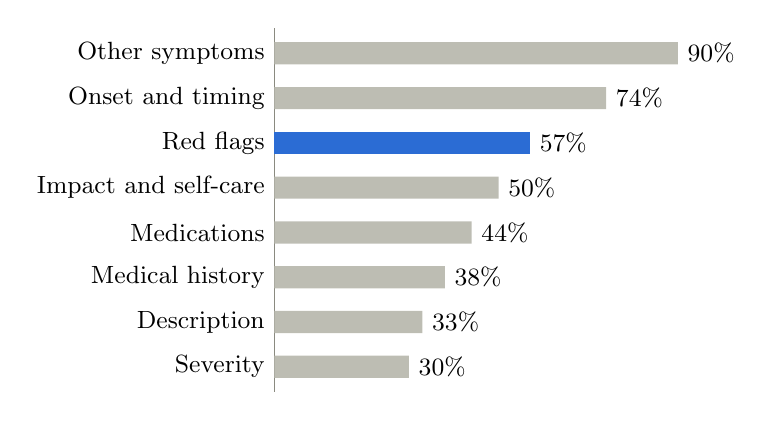
\begin{tikzpicture}
\begin{axis}[
  xbar, width=0.6\columnwidth, height=6.2cm, bar shift=0pt,
  xmin=0, xmax=100, bar width=8pt,
  symbolic y coords={Severity,Description,Medical history,Medications,Impact and self-care,Red flags,Onset and timing,Other symptoms},
  ytick={Severity,Description,Medical history,Medications,Impact and self-care,Red flags,Onset and timing,Other symptoms}, y tick label style={font=\small},
  xtick=\empty, axis x line=none, axis y line*=left,
  y axis line style={draw=edge}, major tick length=0pt,
  nodes near coords={\pgfmathprintnumber{\pgfplotspointmeta}\%},
  nodes near coords style={font=\small, anchor=west},
  enlarge y limits=0.08, clip=false,
]
\addplot[fill=muted, draw=none] coordinates {
  (90,Other symptoms) (74,Onset and timing) (50,Impact and self-care)
  (44,Medications) (38,Medical history) (33,Description) (30,Severity)};
\addplot[fill=accent, draw=none] coordinates {(57,Red flags)};
\end{axis}
\end{tikzpicture}
\caption{Share of the 250 rows whose clinician questions touch each topic, by keyword tagging. Clinicians ask about other symptoms in 90\% of messages, but about severity in only 30\%. Blue: red-flag screening, the safety check every model output must match.}
\label{fig:topics}
\end{figure}

% ---------------------------------------------------------------------------
\section{Evaluation and Error Analysis}

We evaluate every output at several levels (Table~\ref{tab:eval}).
The clinician answers in the dataset are the main reference.

\begin{table*}[t]
\centering\small
\begin{tabularx}{\textwidth}{@{}L{2.9cm}L{5.4cm}L{1.9cm}Y@{}}
\toprule
\textbf{Level} & \textbf{Metric} & \textbf{Task} & \textbf{What it tells us} \\
\midrule
Against clinician answer & Clinician Questions Matched (recall) & Questions & Share of the clinician's questions that the model also asked \\
Against clinician answer & Clinician Reply Coverage & Reply & Share of the points in the clinician's reply that the model covers \\
Automatic, no reference & Topic coverage (8 topics), red-flag screening & Both & If the output covers the key clinical areas \\
Automatic, no reference & Question count, repeated questions, agreement with other models & Questions & If the list is the right size and not repetitive \\
Automatic, no reference & Reading grade level, word count, empathy, emergency advice, referral to care team & Reply & If the reply is readable and has the safety parts \\
Chart grounding & Unsupported mentions, ignored chart items & Both & If the output invents a drug or condition, or misses a relevant one \\
LLM judge & 1--5 scores: relevance, comprehensiveness, safety, clarity, empathy & Both & A quick qualitative score \\
Clinician rating & 1--5 scores: fluency, coherence, relevance, factual correctness, completeness, safety & Both & Blind human judgment from the rating page \\
Multi-turn & Coverage after each turn, turns until advice, warning sign caught & Conversation & How fast and how safely the model gathers facts \\
\bottomrule
\end{tabularx}
\caption{Evaluation levels and metrics.}
\label{tab:eval}
\end{table*}

\paragraph{One-to-one matching.}
The current matcher lets one broad model question count for two clinician questions.
This makes the recall too high.
We will pair the questions one-to-one with the Hungarian algorithm over a TF-IDF similarity matrix.
Each clinician question can then match at most one model question.
We will hand-check 50 matched pairs ourselves and report how many are correct.

\paragraph{Chart grounding.}
We parse each chart summary into a problem list and a medication list.
From all 227 charts, we build a lexicon of drug and condition names.
Then we flag two things in each output: a drug or condition that is not in this patient's chart, and a chart medication that relates to the symptom but is not mentioned.
We test the check on the clinician replies first. They should get few flags.

\paragraph{Results over the dataset.}
Today the app scores one message at a time.
We will add a summary page over all messages.
For each model and metric, it shows the mean with a 95\% bootstrap confidence interval.
A paired test (Wilcoxon signed-rank) on per-message scores shows if one model really beats another.
The page also splits the results by age group, sex, topic, and message length.

\paragraph{Metric agreement (RQ3).}
We compute the rank correlation (Spearman) between the automatic metrics, the reference-based scores, and the judge scores.
As a sanity check, we also score the clinician's own reply with the same metrics and judge.
A good metric should give it a high score.

\paragraph{Clinician ratings.}
The app has a blind rating page.
It shows outputs as Model A, B, and C in random order.
Raters score six dimensions from 1 to 5.
The summary page will report rater agreement (Krippendorff's alpha) and compare the ratings with the automatic scores.

\paragraph{Error analysis.}
We will review all low-scoring outputs and sort each error into one of these types:
\begin{enumerate}
  \item Missed red flag (for example, no question about chest pain when it matters)
  \item Hallucination (a fact that is not in the message or chart)
  \item Unsafe advice (a diagnosis or a change in treatment)
  \item Ignored chart context (for example, a drug the patient already takes)
  \item Too long, too hard to read, or repetitive
  \item Format failure (no list, cut-off output)
\end{enumerate}
The subgroup splits show where models fail more often.

% ---------------------------------------------------------------------------
\section{Interactive System Design}

The system is a Django web app, and a first version already runs (Figure~\ref{fig:system}).
It has six pages:
\begin{itemize}
  \item \textbf{Compare:} pick a message, a task, and models, then generate.
  \item \textbf{Results:} see outputs side by side, with score tiles, metric bars, and the clinician's answer. Download a CSV.
  \item \textbf{Rate:} score outputs blind, 1--5 on six dimensions, with a comment.
  \item \textbf{Dataset:} add, edit, search, import, and export messages.
  \item \textbf{Chat:} have a multi-turn chat with one model. The user plays the patient.
  \item \textbf{Help:} read how each metric works.
\end{itemize}

\paragraph{Reliability.}
The app retries a failed model call up to 3 times.
A Retry button reruns only the failed models.
A mock mode gives fake outputs at no cost, for demos without an API key.

\paragraph{Work to add this term.}
\begin{itemize}
  \item \textbf{Compare page:} the three baselines appear as extra ``models''. A switch turns the chart summary on or off.
  \item \textbf{Results page:} chart-grounding flags under each output, and one-to-one question matching.
  \item \textbf{New summary page:} results over all messages, with confidence intervals, paired tests, and subgroup splits.
  \item \textbf{Chat page:} a simulated-patient mode that runs a whole conversation for a chosen message and scores it turn by turn.
\end{itemize}

\begin{figure}[t]
\centering
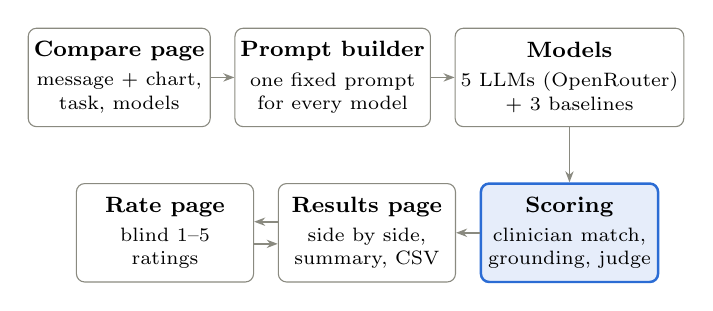
\begin{tikzpicture}[
  font=\footnotesize,
  box/.style={draw=edge, rounded corners=3pt, align=center, minimum width=2.25cm, minimum height=1.25cm, inner sep=2pt},
  main/.style={box, draw=accent, fill=accent!12, line width=0.9pt},
  arr/.style={-{Stealth[length=4pt]}, draw=edge, line width=0.6pt},
  node distance=0.32cm and 0.3cm,
]
\node[box] (compare) {\textbf{Compare page}\\[1pt]\scriptsize message + chart,\\[-1pt]\scriptsize task, models};
\node[box, right=of compare] (prompt) {\textbf{Prompt builder}\\[1pt]\scriptsize one fixed prompt\\[-1pt]\scriptsize for every model};
\node[box, right=of prompt] (models) {\textbf{Models}\\[1pt]\scriptsize 5 LLMs (OpenRouter)\\[-1pt]\scriptsize + 3 baselines};
\node[main, below=0.7cm of models] (score) {\textbf{Scoring}\\[1pt]\scriptsize clinician match,\\[-1pt]\scriptsize grounding, judge};
\node[box, left=of score] (results) {\textbf{Results page}\\[1pt]\scriptsize side by side,\\[-1pt]\scriptsize summary, CSV};
\node[box, left=of results] (rate) {\textbf{Rate page}\\[1pt]\scriptsize blind 1--5\\[-1pt]\scriptsize ratings};
\draw[arr] (compare) -- (prompt);
\draw[arr] (prompt) -- (models);
\draw[arr] (models) -- (score);
\draw[arr] (score) -- (results);
\draw[arr] ([yshift=4pt]results.west) -- ([yshift=4pt]rate.east);
\draw[arr] ([yshift=-4pt]rate.east) -- ([yshift=-4pt]results.west);
\end{tikzpicture}
\caption{Every model gets the same input and is scored the same way. The rate page shows saved runs without model names; the scores return to the results page.}
\label{fig:system}
\end{figure}

\begin{table*}[t]
\centering\small
\begin{tabularx}{\textwidth}{@{}L{3.6cm}L{4.6cm}Y@{}}
\toprule
\textbf{Challenge} & \textbf{Why it matters} & \textbf{Our plan} \\
\midrule
Few human ratings & Human ratings take time to collect & The clinician answers in the dataset are the main reference. Ratings from the rating page add to it. \\
Word-overlap metrics miss paraphrases & Scores can be too low for good outputs & Use one-to-one matching and hand-check a sample of matches. Report the judge next to it. \\
Simulated patients can drift & The patient model may invent facts & Tell it to answer only from the message and chart. Read a sample of conversations. \\
API cost and rate limits & Five models $\times$ two tasks $\times$ two settings, plus conversations, is many calls & Save every output and reuse it. Build and test the baselines and statistics in mock mode, with no API calls. \\
Models change or retire & Results must be repeatable & Save the exact model ID and date with every run. \\
Small, unbalanced dataset & Results may not generalize & Report confidence intervals and subgroup results. \\
\bottomrule
\end{tabularx}
\caption{Anticipated challenges and how we will handle them.}
\label{tab:challenges}
\end{table*}

\begin{figure*}[t]
\centering
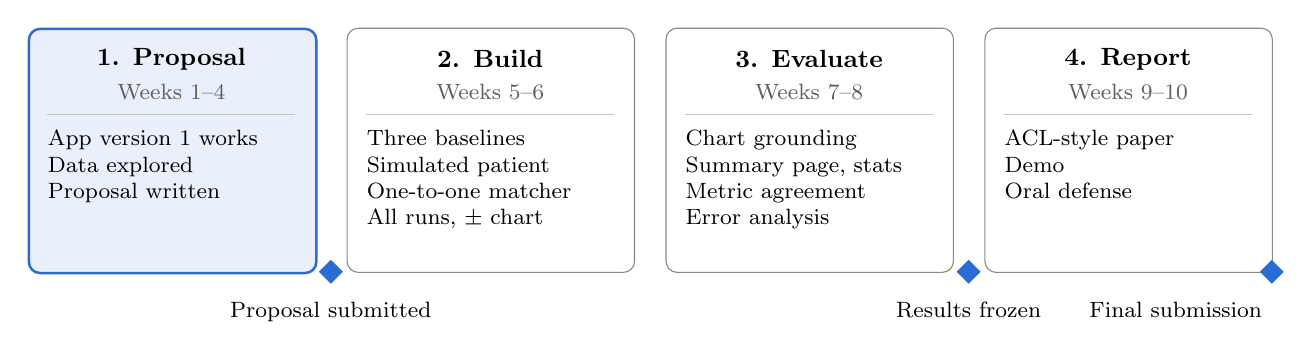
\begin{tikzpicture}[
  font=\small,
  phase/.style={draw=edge, rounded corners=4pt, minimum width=3.65cm, minimum height=3.1cm, anchor=north west},
  gate/.style={diamond, fill=accent, inner sep=2.2pt},
]
\foreach \i/\name/\weeks/\a/\b/\c/\d in {
  0/1. Proposal/Weeks 1--4/App version 1 works/Data explored/Proposal written/,
  1/2. Build/Weeks 5--6/Three baselines/Simulated patient/One-to-one matcher/{All runs, $\pm$ chart},
  2/3. Evaluate/Weeks 7--8/Chart grounding/{Summary page, stats}/Metric agreement/Error analysis,
  3/4. Report/Weeks 9--10/ACL-style paper/Demo/Oral defense/} {
  \pgfmathsetmacro{\x}{\i*4.05}
  \ifnum\i=0
    \node[phase, draw=accent, fill=accent!10, line width=0.9pt] at (\x,0) {};
  \else
    \node[phase] at (\x,0) {};
  \fi
  \node[font=\small\bfseries] at (\x+1.825,-0.4) {\name};
  \node[text=quiet, font=\footnotesize] at (\x+1.825,-0.82) {\weeks};
  \draw[edge!50] (\x+0.25,-1.1) -- (\x+3.4,-1.1);
  \node[anchor=north west, align=left, font=\footnotesize, inner sep=0pt] at (\x+0.25,-1.3) {\a\\\b\\\c\\\d};
}
\node[gate] at (3.85,-3.1) {};
\node[gate] at (11.95,-3.1) {};
\node[gate] at (15.8,-3.1) {};
\node[font=\footnotesize, below=3pt] at (3.85,-3.25) {Proposal submitted};
\node[font=\footnotesize, below=3pt] at (11.95,-3.25) {Results frozen};
\node[font=\footnotesize, below=3pt, anchor=north east] at (15.8,-3.25) {Final submission};
\end{tikzpicture}
\caption{Four phases, three gates: proposal, frozen results, final submission.}
\label{fig:plan}
\end{figure*}

% ---------------------------------------------------------------------------
\section{Ethical, Privacy, Fairness, and Safety Considerations}

\begin{itemize}
  \item \textbf{Privacy.} The app sends text to outside model providers. So we use only de-identified data. The charts show age ranges, not birth dates, and no names of real patients. We will not enter real patient data in the app, including the chat page.
  \item \textbf{Safety.} The outputs are not medical advice, and the app says so on the help and chat pages. The tool is for research and evaluation. It does not send anything to patients.
  \item \textbf{Fairness.} 74\% of the rows are female, so results may not hold for other groups. We will report results by sex and age group and state this limit.
  \item \textbf{Judge bias.} An LLM judge can prefer outputs from its own model family. By default the judge is an OpenAI model, which is also a candidate. We will report this and compare judge scores with the reference-based scores.
  \item \textbf{Automation bias.} A clinician may trust a fluent draft too much. High scores in our study do not mean a model is safe to use without review.
  \item \textbf{Metric limits.} Keyword and overlap metrics can reward the wrong output. We will show where they disagree with the clinician reference answers.
\end{itemize}

% ---------------------------------------------------------------------------
\section{Challenges and Plan}

Table~\ref{tab:challenges} lists the main challenges.
The plan has four phases over the 10-week term (Figure~\ref{fig:plan}).
API runs are the main cost.
So we run each model once per setting, save all outputs, and build the analysis on the saved outputs.


% ---------------------------------------------------------------------------
\section{Division of Responsibilities}

We are a team of three.
Each member leads one part of the system (Table~\ref{tab:roles}) and also helps with the other parts.
The parts connect.
Jialin's turn-by-turn scoring uses Sudarshan's question matcher.
The summary page reports results from Lubna's runs, Jialin's conversations, and the rating page.

\begin{table}[!h]
\centering\small
\begin{tabularx}{\columnwidth}{@{}YL{1.55cm}@{}}
\toprule
\textbf{Area} & \textbf{Lead} \\
\midrule
Comparison app, model calls, dataset import, LLM judge, blind rating page & Lubna \\
Chart on/off ablation runs (RQ2) & Lubna \\
Initial data exploration & Lubna \\
Multi-turn chat, simulated patient, turn-by-turn scoring (RQ4) & Jialin \\
Non-LLM baselines: checklist, TF-IDF, BM25 (RQ1) & Sudarshan \\
One-to-one question matcher & Sudarshan \\
Chart-grounding check & Sudarshan \\
Summary page: confidence intervals, paired tests, subgroups, metric agreement (RQ3) & Sudarshan \\
Proposal, error analysis, report, and demo & All \\
\bottomrule
\end{tabularx}
\caption{Division of responsibilities.}
\label{tab:roles}
\end{table}

\section*{GenAI Use Disclosure}

GenAI was used in polishing the contents of this document.

\end{document}
